% Drawing 156-9/01-2 -- folder 156-9, batch 01, archive page 2 (PDF page 3).
% Transcription: un graphe au crayon et à l'encre, de sommets S (en haut), LS, M (cerclés), SF, E, MF, EM (cerclé) et Mq (en bas) : S est relié à M par un arc épais et à LS ; SF est au centre, relié à S, à E et à MF ; M est relié à MF par un arc ; MF est relié à EM et à Mq ; LS est relié à E puis à EM. À côté : « DEQFLMPS » et dessous « Mq, Div, v, p ».
% Kind: graph on S, LS, M, SF, E, MF, EM, Mq. Method 2 (schematic redraw from the facsimile). Status: ok.
% Notes: Pencil and ink graph: S at the top joined to M by a thick arc and to LS; SF in the centre joined to S, E and MF; M joined to MF by an arc; MF to EM and Mq; LS to E, E to EM; LS, M and EM ringed. Beside it "DEQFLMPS" and under it "Mq, Div, v, p".
% Coordinates: 1 unit = 1 mm = 1/100 of the crop width (bbox in page fractions: [0.2, 0.37, 0.55, 0.52]).
% Redrawn by Claude (claude-opus-5-5), issue #73, 2026-11-07; not checked by a human; not compiled (no TeX in the session).
% Rights: reproduces part of the work -- behind RENDER_TRANSCRIPTS, never published by itself.
\documentclass[tikz,border=3pt]{standalone}
\usepackage{amsmath,amssymb}
\usetikzlibrary{patterns,arrows.meta}
\tikzset{pencil/.style={black!45}, struck/.style={black!35}, mark/.style={circle,draw,inner sep=1.3pt}, pt/.style={circle,fill,inner sep=0.9pt}, opt/.style={circle,draw,fill=white,inner sep=1.1pt}}
\begin{document}
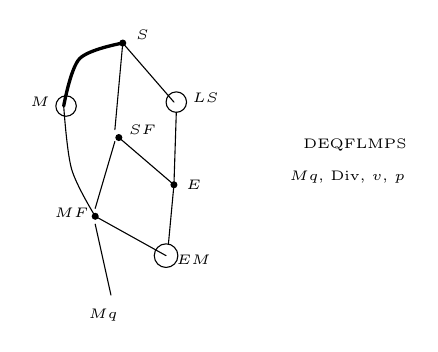
\begin{tikzpicture}[x=1mm,y=1mm,line cap=round,line join=round,font=\scriptsize]
\draw[very thick] plot[smooth, tension=0.55] coordinates {(31.5,-14) (26,-16) (24,-22)};
\draw (31.5,-14) -- (38,-21.5);
\draw (31.5,-14) -- (30.5,-25);
\draw (31,-26) -- (38,-32);
\draw (30.5,-26.5) -- (28,-35);
\draw plot[smooth, tension=0.55] coordinates {(24,-22) (25,-30) (28,-36)};
\draw (28,-36) -- (37,-41);
\draw (28,-37) -- (30,-46);
\draw (38.3,-22.8) -- (38,-32);
\draw (38,-32) -- (37.3,-39.5);
\node[pt] at (31.5,-14) {};
\node[pt] at (31,-26) {};
\node[pt] at (38,-32) {};
\node[pt] at (28,-36) {};
\draw (38.3,-21.5) circle[radius=1.3];
\draw (24.3,-22) circle[radius=1.3];
\draw (37,-41) circle[radius=1.5];
\node[inner sep=1pt] at (34,-13) {\tiny $S$};
\node[inner sep=1pt] at (42,-21) {\tiny $LS$};
\node[inner sep=1pt] at (21,-21.5) {\tiny $M$};
\node[inner sep=1pt] at (34,-25) {\tiny $SF$};
\node[inner sep=1pt] at (40.5,-32) {\tiny $E$};
\node[inner sep=1pt] at (25,-35.5) {\tiny $MF$};
\node[inner sep=1pt] at (40.5,-41.5) {\tiny $EM$};
\node[inner sep=1pt] at (29,-48.5) {\tiny $Mq$};
\node[inner sep=1pt] at (61,-27) {\tiny DEQFLMPS};
\node[inner sep=1pt] at (60,-31) {\tiny $Mq$, Div, $v$, $p$};
\end{tikzpicture}
\end{document}
